\documentclass{beamer}
\usepackage{amsfonts,amsmath,oldgerm}
\usepackage{xspace}
\usepackage{bbm}
\usepackage{tabularx}
\usepackage{booktabs}
\usepackage{adjustbox}
\usetheme{sintef}
\usepackage{tikz}

\usepackage{xeCJK}
\usepackage{multirow}
% table
\usepackage{booktabs}
\usepackage{threeparttable}
% \input{bring-your-own/arXiv-2311.07850v1/math_commands.tex}
% \usepackage{tabularx}

\newcommand{\testcolor}[1]{\colorbox{#1}{\textcolor{#1}{test}}~\texttt{#1}}

% newcommand for red text
\newcommand{\red}[1]{\textcolor{red}{#1}}
\newcommand{\dataname}{\textsc{Knot}\xspace}
\newcommand{\datanameE}{\textsc{Knot}-E\xspace}
\newcommand{\datanameS}{\textsc{Knot}-S\xspace}
\newcommand{\datanameI}{\textsc{Knot}-I\xspace}
% \newcommand{\datanameE}{K{\small NOT}-E\xspace}
% \newcommand{\datanameS}{K{\small NOT}-S\xspace}
% \newcommand{\datanameI}{K{\small NOT}-I\xspace}

\usepackage{colortbl}
\definecolor{'sgreen'}{HTML}{F3FADF} 
\definecolor{'sred'}{HTML}{FFEAE8}

\usefonttheme[onlymath]{serif}

\titlebackground*{assets/background}

\newcommand{\hrefcol}[2]{\textcolor{cyan}{\href{#1}{#2}}}
\newcommand*{\rom}[1]{\expandafter\@slowromancap\romannumeral #1@}


\title{Evaluation of Reasoning Ability of Retrieval-based Language Models}
% \course{Master's Degree in Computer Science}
\author{Yantao Liu}
% \IDnumber{1234567}
\date{\today}


\begin{document}
\maketitle

\section{Introduction}
\begin{frame}
\frametitle{What is Retrieval-based Language Models?}
    % color blue
    Retrieval-based LMs = Retrieval + LMs
    \begin{itemize}
        \item It is a \textbf{Language Model} \\
        \begin{center}
            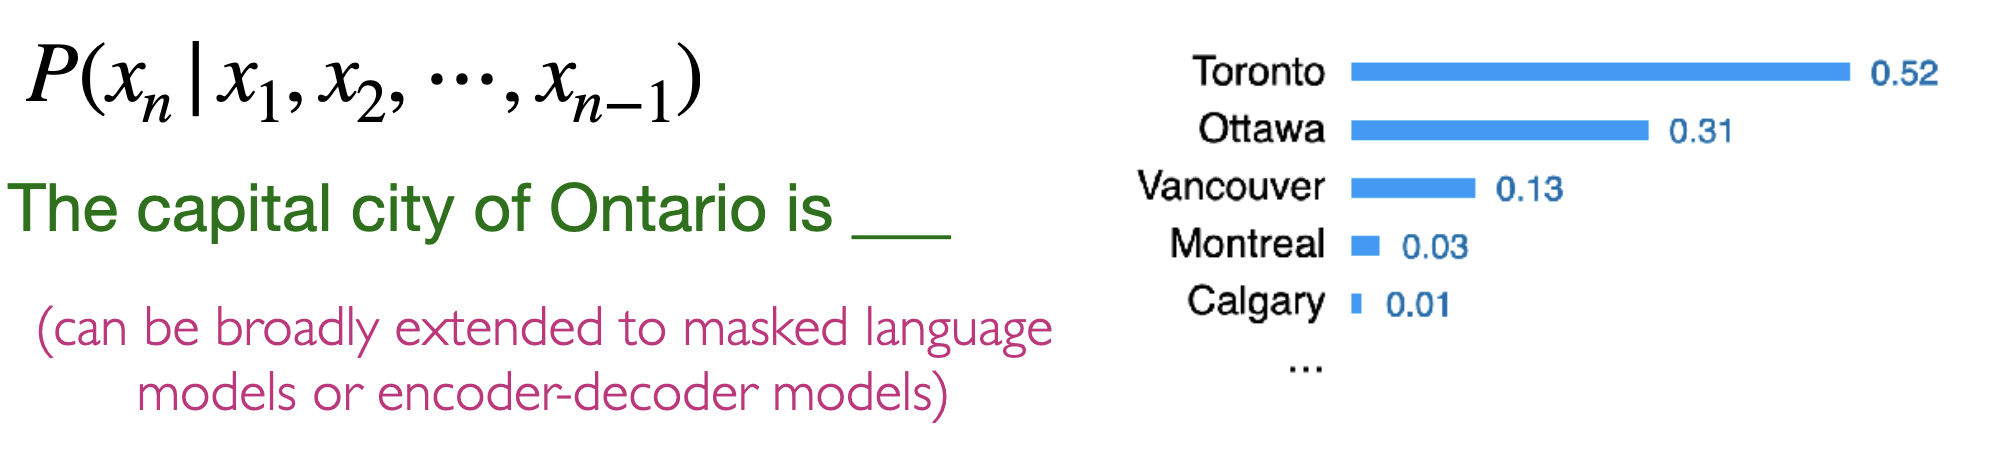
\includegraphics[width=0.6\textwidth]{figure/lm.png}
        \end{center}
        \item It retrieves from an \textbf{external knowledge source} at inference time
        \begin{center}
            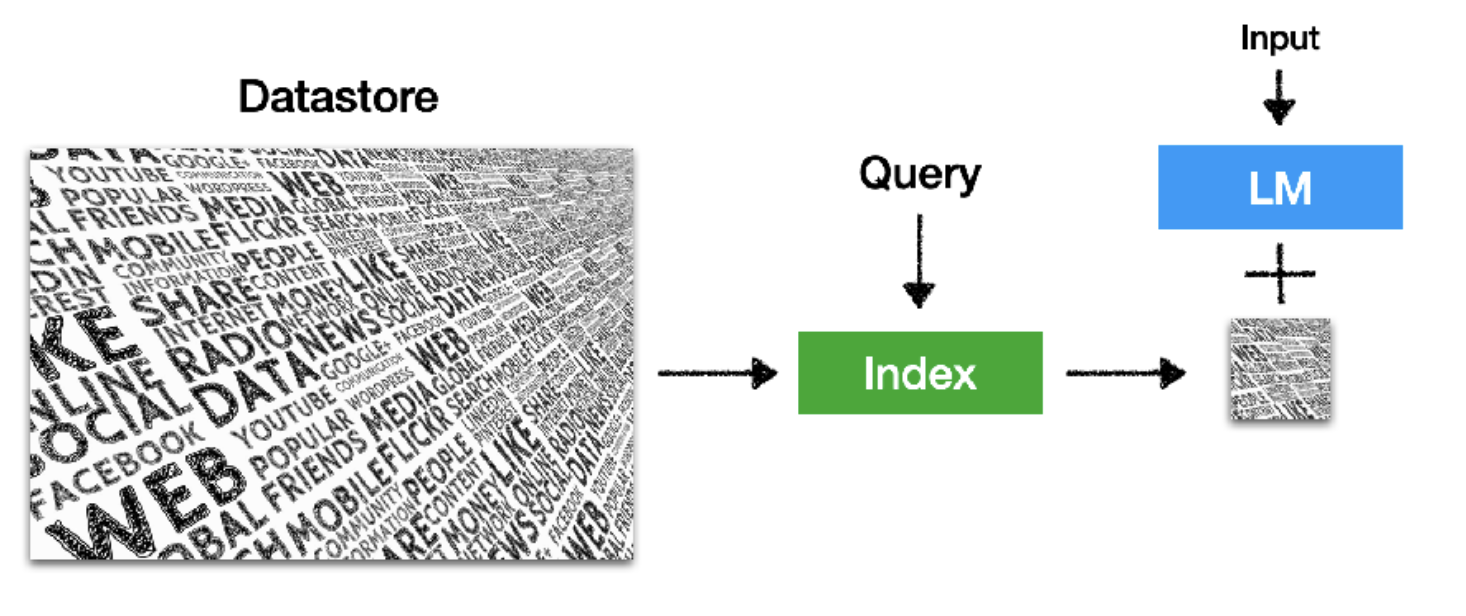
\includegraphics[width=0.6\textwidth]{figure/retrieval.png}
        \end{center}
    \end{itemize}
\end{frame}

\begin{frame}
    \frametitle{Why do we care about the reasoning ability of Retrieval-based LMs?}
    \begin{itemize}
        \item It is a \textbf{Language Model} \\
         --> It already has internal knowledge
        \item It retrieves from an \textbf{external knowledge source} at inference time \\
         --> External knowledge will also be integrated into the model
        \item This leads to the following questions:
    \end{itemize}
    \begin{block}{Interactions between internal and external knowledge}
        \textbf{RQ1:} How well can LMs integrate external knowledge with internal knowledge? \textit{\red{ACL 2023}} \\
        \textbf{RQ2:} How well can LMs reason about conflicting external knowledge? \textit{\red{COLING 2024}} \\
        \textbf{RQ3:} How well can LMs reason about new real-world external knowledge? \textit{\red{ICLR 2024}}
    \end{block}
\end{frame}


\section{KoRC: Knowledge Oriented Reading Comprehension (ACL 2023)}

\begin{frame}
\frametitle{Background}
\begin{itemize}
    \item Existing QA datasets focus on either:
    \begin{itemize}
        \item Extracting knowledge from passages (e.g., SQuAD, HotpotQA).
        \item Evaluating internal knowledge of LLMs (e.g., TriviaQA, Natural Questions).
    \end{itemize}
\end{itemize}

\end{frame}

\begin{frame}
\frametitle{Motivation}
\begin{columns}
    \column{0.5\textwidth}
    % Existing QA datasets either focus on extracting knowledge from the passage (SQuAD, HotpotQA) or examining the internal knowledge of LLMs (TriviaQA, Natural Questions) \\
    \textbf{Object:} Evaluate the ability of LLMs to integrate knowledge from external sources with its internal knowledge.
    \begin{enumerate}
        \item Answering questions requires multiple-hop reasoning
        \item The reasoning chain scatters in both the given \textbf{passage} and the \textbf{Internal Knowledge} of LLMs
        \item Anonymized question entity in the passage to avoid information leakage
        % \item Board coverage of knowledge: Use Knowledge Base and LLM to generate questions
        % \item Flexible evaluation: Allow one questions to have multiple correct answers
    \end{enumerate}
    \column{0.45\textwidth}
    \vspace*{-0.2cm}
    \begin{center}
        \includegraphics[width=0.8\textwidth]{figure/korc-intro.pdf}
    \end{center}
\end{columns}
\end{frame}


\begin{frame}
\frametitle{Dataset Construction}
\begin{center}
    \includegraphics[width=\textwidth]{figure/korc-construction.pdf}
\end{center}
\end{frame}

\begin{frame}
\frametitle{Dataset Construction - Document Preparation}
\begin{columns}
    \column{0.5\textwidth}
    \begin{itemize}
        \item Align document to a background knowledge base
        \item Entity linking
        \item Document Relation Extraction
    \end{itemize}
    \column{0.45\textwidth}
    % \vspace*{-1.7cm}
    \begin{center}
        \includegraphics[width=0.8\textwidth]{figure/korc-doc-prep.pdf}
    \end{center}
\end{columns}    
\end{frame}

\begin{frame}
\frametitle{Dataset Construction - Reasoning Chain Preparation}

\begin{columns}
    \column{0.5\textwidth}
    \begin{itemize}
        \item Relation Compositional Rules Mining
        \item Reasoning Chain Extraction
    \end{itemize}
    \column{0.45\textwidth}
    % \vspace*{-1.7cm}
    \begin{center}
        \includegraphics[width=0.65\textwidth]{figure/korc-rule-prep.pdf}
    \end{center}
\end{columns}
\end{frame}

\begin{frame}
\frametitle{Dataset Construction - Data Annotation}
\begin{columns}
    \column{0.5\textwidth}
    \begin{itemize}
        \item Preventing Bypass Background Knowledge: Question Filtering
        \item Prevent Bypassing Document: Entity Name Anonymization
        \item Question Generation: Template or Humann or LLMs
    \end{itemize}
    \column{0.45\textwidth}
    % \vspace*{-1.7cm}
    \begin{center}
        \includegraphics[width=0.8\textwidth]{figure/korc-data-anon.pdf}
    \end{center}
\end{columns}
\end{frame}

\begin{frame}
\frametitle{Dataset Analysis}
\begin{itemize}
    \item Dataset Splitting
    \begin{center}
    \begin{table}[tbp]
        \centering
        \scalebox{0.76}{
        \setlength{\tabcolsep}{6pt}
        \begin{tabular}{lcccccccccccccc}
        \toprule
        Split & Train & Valid & Test-ID & Test-OOD & All\\
        \midrule
        \#Document (Unique) & $7,260$ $(2,332)$ & $4,637$ $(2,074)$ & $546$ $(546)$ & $516$ $(516)$ & $9,086$ $(3,291)$ \\
        \#Relation (Unique) & $208$ $(117)$ & $185$ $(113)$ & $121$ $(90)$ & $162$ $(111)$ & $212$ $(119)$ \\
        \#Question & $18,945$ & $7,574$ & $3,432$ & $1,853$ & $31,804$ \\
        % Average Answer per Question & 3.6 & 3.6 & 4.8 & 2.6 & 3.7 \\
        Average Hops per Answer & $2.80$ & $2.80$ & $2.84$ & $2.81$ & $2.80$ \\
        \bottomrule
        \end{tabular}
        }
        % \caption{Statistics of the final version of KoRC.
        % Unique documents is the number of documents before anonymization.
        % Unique relation considers the inverse relation the same as the forward relation.
        % They are shown in the parenthesis.
        % }
        \label{tab:data}
    \end{table}
    \end{center}
    \item Dataset Distribution
    \begin{center}
        \includegraphics[width=0.7\textwidth]{figure/knot-trigram.pdf}
    \end{center}
\end{itemize}
\end{frame}

\begin{frame}
\frametitle{Main Results on Human Annotated KoRC (KoRC-H)}

\begin{columns}
    \column{0.5\textwidth}
    \begin{itemize}
        \item The best results are achieved by fine-tuning Flan-T5-XXL
        \begin{itemize}
            \item Store background knowledge in parameters
        \end{itemize}
        \item The secondly best results are achieved by models with abilities to access background knowledge
        \begin{itemize}
            \item Access external knowledge such as text (RAG) and KB (EmbedKGQA)
        \end{itemize}
        \item LLMs at that time\footnote{The experiments are conducted at Nov 2022} are not good at integrating external knowledge with internal knowledge
    \end{itemize}
    \column{0.5\textwidth}
    \begin{table}[!th]
\centering
\scalebox{0.80}{
\begin{threeparttable}
\setlength{\tabcolsep}{3.2pt}
\begin{tabular}{lccccccc}
\toprule
\multirow{2}{*}{\textbf{KoRC-H}} & \multicolumn{3}{c}{P-ACC} & \multicolumn{3}{c}{P-F1} \\
\cmidrule(r){2-4}\cmidrule(lr){5-7}
& ID & OOD & Mean & ID & OOD & Mean \\
\midrule
BART-base
& $50.3$ & $24.9$ & $41.4$
& $52.9$ & $30.2$ & $44.9$ \\
Flan-T5-base 
& $33.5$ & $24.0$ & $30.2$
& $35.8$ & $27.5$ & $32.9$ \\
Flan-T5-XXL 
& $\mathbf{63.8}$ & $\mathbf{32.3}$ & $\mathbf{52.8}$
& $65.8$ & $\mathbf{37.2}$ & $\mathbf{55.8}$ \\
\midrule
GPT-3 
&  $18.2$ &  $24.6$ & $20.5$
&  $22.2$ & $30.2$ & $25.0$ \\
GLM-130B
&  $9.9$ &  $14.9$ & $11.6$
&  $12.7$ & $18.8$ & $14.8$ \\
\midrule
RAG-seq
& $61.7$ & $25.9$ & $49.2$
& $63.7$ & $30.0$ & $51.9$ \\
RAG-token 
& $57.4$ & $23.5$ & $45.5$
& $59.1$ & $27.2$ & $47.9$ \\
\midrule
EmbedKGQA 
& $61.2$ & $21.9$ & $47.4$ 
& $\mathbf{68.3}$ & $28.9$ & $54.5$ \\
EmbedKGQA$^*$ 
& $34.0$ & $13.6$ & $26.9$
& $41.6$ & $21.8$ & $34.6$ \\
TransferNet 
& $32.7$ & $12.9$ & $25.8$
& $37.7$ & $16.6$ & $30.3$ \\
\bottomrule
\end{tabular}
\end{threeparttable}
}
\label{tab:baseline}
\end{table}
\end{columns}
\end{frame}


\section{Untangle the KNOT (COLING 2024)}
\begin{frame}
\frametitle{Background}
\begin{itemize}
    \item LLMs' knowledge is easily outdataed and hard to update 
    \begin{columns}
        \column{0.5\textwidth}
        \begin{center}
            
\includegraphics[width=\textwidth]{figure/knot-twitter-ceo-example.png}
        \end{center}
        \column{0.5\textwidth}
        \begin{center}
            
\includegraphics[width=\textwidth]{figure/knot-twitter-ex-by-google.png}
        \end{center}
    \end{columns}


    % \item Existing \textbf{knowledge editing} methods are still NOT scalable
    % \item The external non-parametric knowledge is hard to be integrated into LLMs
\end{itemize}
\end{frame}

\begin{frame}
\frametitle{Object}
\begin{columns}[t]
    \column{0.5\textwidth}
    \begin{itemize}
        \item \textbf{Object:} Evaluate the ability of LLMs to reason about conflicting external knowledge
        \begin{itemize}
            \item Categories the reason skills into \textbf{3} levels
            \item \textbf{Knot-Simple}: requires LLMs directly extract the conflicting knowledge from the given passage
            \item \textbf{Knot-Explicit} and \textbf{Knot-Implicit}: requires LLMs to reason with the conflicting external knowledge and its internal knowledge
        \end{itemize}
    \end{itemize}
    \column{0.50\textwidth}
    \vspace*{-2.35cm}
    \begin{center}
        \includegraphics[width=0.8\textwidth]{figure/knot-intro.pdf}
    \end{center}
\end{columns}
\end{frame}


\begin{frame}
\frametitle{Dataset Construction}
\begin{center}
    \includegraphics[width=\textwidth]{figure/knot-construction.pdf}
\end{center}
\end{frame}


\begin{frame}
    \frametitle{Dataset Construction - Knowledge Saliency Calculation}
    \begin{itemize}
        \item Calulate the saliency of each node in Wikidata by PageRank
        \item Select the top-$1\%$ entity nodes as topic enitty $e^t$ 
    \end{itemize}
    \begin{center}
        \includegraphics[width=0.85\textwidth]{figure/knot-construction.pdf}
    \end{center}
\end{frame}

\begin{frame}
    \frametitle{Data Construction - Document Generation}
    \begin{itemize}
        \item For each topic entity $e_t$, sample a subgraph as the ego network from Wikidata
        \item Swap one of the neighbors $e$ in the ego network with a conflicting node $e'$ 
        \item Then prompt \texttt{gpt-3.5-turbo} to generate a document based on the ego network
    \end{itemize}
    \begin{center}
        \includegraphics[width=0.75\textwidth]{figure/knot-construction.pdf}
    \end{center}
\end{frame}

\begin{frame}
    \frametitle{Data Construction - Question Generation}
    \begin{columns}[t]
        \column{0.60\textwidth}
        \begin{itemize}
            \item \textbf{Knot-S}: ``Which entity has relation \texttt{$r$} with \texttt{$e_t$}?''
            \item \textbf{Knot-E}: ``Whcih entity has relation $r_2$ with the entity that has relation $r_1$ with $e_t$?''
            \item \textbf{Knot-I}
            \begin{itemize}
                \item Decomposition Rule: $r = r_1 + \dots + r_n$
                \item First hop $r_1$ is in provided document \\ \texttt{Messi $\xrightarrow{playsFor}$ Inter Miami}
                \item And the remaining hops are the background knowledge \\ \texttt{Inter Miami $\xrightarrow{LocatedIn}$ Miami}
                \item Question: ``Which entity has relation \texttt{$r$} with \texttt{$e_t$}?''
            \end{itemize}
        \end{itemize}
        \column{0.45\textwidth}
        \begin{center}
            \vspace*{-1cm}
            \includegraphics[width=0.9\textwidth]{figure/knot-three.pdf}
        \end{center}
    \end{columns}
\end{frame}

\begin{frame}{Dataset Analysis}
    \begin{columns}[t]
        \column{0.5\textwidth}
        \begin{itemize}
            \item General Statistics
            \begin{itemize}
                \item A.S stands for average saliency ranking in percentage
            \end{itemize}
            \item Consistency between saliency and parametric knowledge
            \begin{itemize}
                \item whether \textbf{salient knowledge in Wikidata} act as a good proxy for \textbf{parametric knowledge of LLMs}
                \item evaluate LLaMA-2-70B-Chat on \dataname without providing the documents (only rely on its memory to answer the questions)
            \end{itemize}
        \end{itemize}
        \column{0.5\textwidth}
        \vspace*{-1cm}
        \begin{table}[t]
            \centering
            \setlength{\tabcolsep}{3pt}
            \scalebox{0.75}{
            \begin{tabular}{lcccc}
            \toprule
            Split                    & \datanameS    & \datanameE      & \datanameI \\ \midrule
            \#Questions for evaluation  & $3,887$       & $1,136$         & $510$           \\
            A.S. of Topic Entity     & $8.66$        & $7.51$          & $5.86$         \\
            A.S. of Answer Entity    & $0.83$        & $0.19$          & $0.18$          \\
            A.S. of Answer in Memory & $0.56$        & $0.18$          & $0.19$          \\
            Average Reasoning Hops   & $1$           & $2$             & $2.7$          \\ 
            \midrule
            \#Questions for training & $603$ & $190$ & $26$ \\
            \bottomrule
            \end{tabular}
            }
            \label{tab:dataset}
        \end{table}
        
        \begin{figure}
            \centering
            \includegraphics[width=0.9\linewidth]{figure/llama-2-70b-chat-wo-psg.pdf}
            \label{fig:llama-2-70b-chat-wo-psg}
        \end{figure}

    \end{columns}
    
\end{frame}


\begin{frame}{Experiments}
    \begin{itemize}
        \item How well can LLMs reason about conflicting external knowledge?
        \begin{itemize}
            \item \textbf{Effect of Reasoning Type:} Knot-Simple v.s. Knot-Explicit v.s. Knot-Implicit
            \item \textbf{Effect of Alignment:} Pre-trained only v.s. Assistant LLMs
        \end{itemize}
        \item How well the existing knowledge editing methods work on \dataname?
        \begin{itemize}
            \item Prompting
            \item Decoding
            \item Fine-tuning
        \end{itemize}
    \end{itemize}
\end{frame}

\begin{frame}
\frametitle{Main Results on \dataname}

\begin{columns}[t]
    \column{0.5\textwidth}
    How well can LLMs reason about conflicting external knowledge?
    \begin{itemize}
        \item Effect of Reasoning Type:
        \begin{itemize}
            \item \datanameS: It is not challenging for capable LLMs to simply extract conflicting knowledge from the given passage
            \item \datanameE and \datanameI: When reasoning skills are required, the performance drops significantly
        \end{itemize}
        % TODO: need to refine the description here
        \item Effect of Alignment:
        \begin{itemize}
            \item 13B variants of LLaMA and LLaMA-2 worse than 7B variants
            \item while, this is not observed in counterparts of assistant LLMs (Alpac, Vicuna, Tulu and LLaMA-2-chat)
        \end{itemize}
        
    \end{itemize}
    \column{0.5\textwidth}
    \vspace*{-2.15cm}
    \begin{table}[t]
        \centering
        \setlength{\tabcolsep}{3pt}
        \scalebox{0.76}{
        \begin{tabular}{llrrrr}
        \toprule
        Type & LLM      & \datanameS & \datanameE & \datanameI \\ \midrule
        \multirow{7}{*}{\rotatebox{90}{Pre-trained\;\ Only}}
        & GPT-J    & $48.57$  & $29.84$   & $18.63$   \\
        & GPT-NeoX   & $55.65$  & $30.72$   & $20.39$   \\
        & LLaMA-7B    & $64.19$  & $38.20$   & $21.18$   \\
        & LLaMA-13B    & $49.65$  & $27.20$   & $17.45$   \\
        & LLaMA-2-7B   & $63.88$  & $35.65$   & $20.59$   \\
        & LLaMA-2-13B  & $77.18$  & $42.52$   & $24.51$   \\
        & LLaMA-2-70B  & $59.63$  & $32.75$   & $20.20$   \\
        \cmidrule(lr){1-5}
        \multirow{11}{*}{\rotatebox{90}{Assistant\;\ LLMs}}
        & GPT-JT   & $60.59$  & $32.57$   & $17.25$   \\
        & GPT-NeoXT   & $70.03$  & $38.73$   & $27.65$   \\
        & Alpaca-7B    & $82.74$  & $46.83$   & $29.22$   \\
        & Alpaca-13B    & $85.82$  & $43.75$   & $28.82$   \\
        & Vicuna-7B    & $75.92$  & $42.43$   & $26.67$   \\
        & Vicuna-13B    & $84.20$   & $46.30$    & $25.29$   \\
        & Tulu-7B     & $86.72$  & $51.50$    & $27.06$   \\
        & Tulu-13B    & $87.34$  & $53.26$   & $26.67$   \\
        & LLaMA-2-7B-Chat   & $90.66$  & $50.18$   & $28.82$   \\
        & LLaMA-2-13B-Chat  & $91.66$  & $53.43$   & $35.88$   \\
        & LLaMA-2-70B-Chat  & $94.93$  & $58.54$   & $38.24$   \\
        \cmidrule(lr){2-5}
        & \texttt{gpt-3.5-turbo}   & $83.66$  & $34.95$   & $10.20$   \\
        & \texttt{text-davinci-003}  & $95.11$  & $63.56$   & $35.49$   \\
        \bottomrule
        \end{tabular}
        }
        \label{tab:main-result}
    \end{table}
\end{columns}
\end{frame}

\begin{frame}
\frametitle{Existing Methods: Prompting}
\begin{columns}[t]
    \column{0.5\textwidth}
    \begin{itemize}
        \item In the main experiment, we adopt the regular Q\&A prompting
        \item \cite{zhou-etal-2023-context} proposed two prompting strategies (\textit{i.e.}, Instr+Opin) for conflicting knowledge
        \item \textbf{Takeaway:} One well-designed strategy on one dataset may not be suitable for another dataset
    \end{itemize}
    \column{0.5\textwidth}
    \vspace*{-0.5cm}
    \begin{figure}
        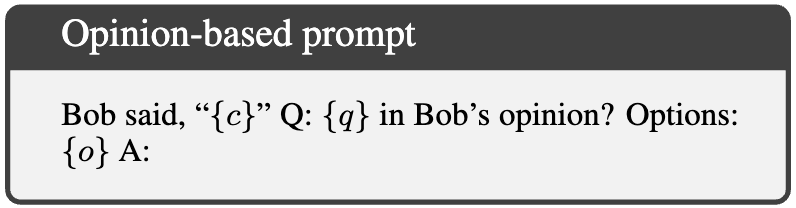
\includegraphics[width=\textwidth]{figure/muhao-prompting.png}
    \end{figure}
    \begin{table}
        \scalebox{0.7}{
        \renewcommand{\arraystretch}{1.2}
        \setlength{\tabcolsep}{3pt}
        \begin{tabular}{lrrrrrr}
        \toprule
         & LLMs                         & \datanameS & \datanameE & \datanameI \\ 
        \midrule
        
        \multirow{5}{*}{\rotatebox{90}{Instr+Opin}}
        
        & LLaMA-7B            & \cellcolor{'sred'} $57.0$ ($-\;\;7.2$)   & \cellcolor{'sgreen'} $40.9$ ($+\;\;2.7$)   & \cellcolor{'sred'}$17.7$ ($-\;\;3.5$)    \\
        & Alpaca-7B           & \cellcolor{'sred'} $78.2$ ($-\;\;4.6$)   &  $46.8$ ($\;\;\;\;0.0$)                        & \cellcolor{'sred'} $26.1$ ($-\;\;3.1$)    \\
        & Vicuna-7B           & \cellcolor{'sred'} $32.6$ ($-43.4$)  & \cellcolor{'sred'} $25.0$ ($-17.4$)    & \cellcolor{'sred'} $12.9$ ($-13.7$)       \\
        & Tulu-7B             & \cellcolor{'sred'} $83.5$ ($-\;\;3.3$)   & \cellcolor{'sred'} $47.6$ ($-\;\;3.9$)     & \cellcolor{'sred'} $26.3$ ($-\;\;0.8$)   \\ 
        % Tulu-13B 88.8 (+1.5)	46.8 (-6.5)	26.7 (0.0)
        &Tulu-13B             & \cellcolor{'sred'} $88.8$ ($+\;\;1.5$)   & \cellcolor{'sred'} $46.8$ ($-\;\;6.5$)     & $26.7$ ($\;\;\;\;0.0$)   \\
        \bottomrule
        \end{tabular}
        }
        \caption{
        Accuracy (\%) with prompting strategies.
        % We show absolute accuracy changes compared with results from main experiment in parenthesis.
        We report Accuracy changes w.r.t main exp in ()
        }
        \label{tab:prompting}
    \end{table}
\end{columns}
\end{frame}



\backmatter
\setbeamertemplate{bibliography item}{[\theenumiv]}
\bibliographystyle{plain}
\bibliography{ref}

\end{document}